\documentclass[11pt]{article}

\usepackage[a4paper,margin=27mm]{geometry}
\usepackage{fontspec}
\usepackage{xeCJK}
\usepackage{unicode-math}
\setmainfont{TeX Gyre Termes}
\setsansfont{TeX Gyre Heros}
\setmonofont{TeX Gyre Cursor}
\setmathfont{TeX Gyre Termes Math}
\setCJKmainfont{Noto Serif CJK SC}
\setCJKsansfont{Noto Sans CJK SC}
\setCJKmonofont{Noto Sans Mono CJK SC}
\usepackage{microtype}
\usepackage{amsthm}
\usepackage{amsmath}
\usepackage{mathtools}
\usepackage{booktabs}
\usepackage{tabularx}
\usepackage{longtable}
\usepackage{array}
\usepackage{enumitem}
\usepackage{graphicx}
\usepackage{tikz}
\usetikzlibrary{arrows.meta,positioning,fit,calc,backgrounds}
\usepackage[numbers,sort&compress]{natbib}
\usepackage{xcolor}
\usepackage{url}
\usepackage{hyperref}
\usepackage[nameinlink,noabbrev]{cleveref}

\hypersetup{
  unicode=true,
  pdftitle={Continuous Convolution Collapse on Indiscrete Arithmetic Orbit Groupoids},
  pdfauthor={Liang Wang},
  pdfsubject={Convention-sensitive convolution on inherited-indiscrete rational-Witt fixed orbits},
  pdfkeywords={arithmetic dynamics, rational Witt vectors, non-Hausdorff groupoids, convolution, quasi-compact support, crossed-product proxy},
  colorlinks=true,
  linkcolor=blue!45!black,
  citecolor=green!35!black,
  urlcolor=blue!55!black
}

\setlength{\parindent}{1.35em}
\setlength{\parskip}{0.25em}
\setlength{\emergencystretch}{3em}
\setlist{nosep,leftmargin=2em}
\renewcommand{\arraystretch}{1.14}
\newcolumntype{Y}{>{\raggedright\arraybackslash}X}
\newcolumntype{P}[1]{>{\raggedright\arraybackslash}p{#1}}

\newtheorem{theorem}{Theorem}[section]
\newtheorem{proposition}[theorem]{Proposition}
\newtheorem{lemma}[theorem]{Lemma}
\newtheorem{corollary}[theorem]{Corollary}
\theoremstyle{definition}
\newtheorem{definition}[theorem]{Definition}
\newtheorem{remark}[theorem]{Remark}

\newcommand{\Borel}{\mathcal B}
\newcommand{\C}{\mathbb C}
\newcommand{\R}{\mathbb R}
\newcommand{\Z}{\mathbb Z}
\newcommand{\Gact}{G_{p,a}^{\mathrm{act}}}
\newcommand{\Gstd}{G_p^{\mathrm{std}}}
\newcommand{\Xpa}{X_{p,a}}
\newcommand{\Cglob}{C_{\mathrm{qc}}^{\mathrm{glob}}}
\newcommand{\CHOp}{C_c^{\mathrm{HOp}}}
\newcommand{\Cfull}{C_{\mathrm{glob}}^{\mathrm{full}}}
\newcommand{\Cred}{C_{\mathrm{glob}}^{\mathrm{red}}}
\newcommand{\Aconst}{A_{\mathrm{const}}}
\newcommand{\supp}{\operatorname{supp}}
\newcommand{\Ind}{\operatorname{Ind}}
\newcommand{\RouteA}{\textsc{Route A}}
\newcommand{\RouteB}{\textsc{Route B}}
\newcommand{\NA}{\textsc{not\_applicable}}
\newcommand{\Diag}{\textsc{diagnostic\_only}}

\title{\textbf{Continuous Convolution Collapse on\\Indiscrete Arithmetic Orbit Groupoids}}
\author{Liang Wang\\
\small School of Artificial Intelligence and Automation\\
\small Huazhong University of Science and Technology\\
\small \href{mailto:wangliang.f@gmail.com}{wangliang.f@gmail.com}}
\date{15 August 2026}

\begin{document}
\maketitle

\begin{abstract}
For every rational prime $p$ and every normalized label $a$, consider the
transformation groupoid of one rational-Witt fixed orbit equipped with its
actual inherited-indiscrete unit topology.  We prove that every continuous
arrow map to a $T_0$ target factors uniquely through real time.  Adding the
open-cover quasi-compact support condition gives a canonical $*$-isomorphism
between the author-defined global algebra $\Cglob(\Gact)$ and ordinary
$C_c(\R)$.  Direct range-fibre convolution and source-fibre calculations
identify the author-defined unit-regular family with the left regular
representation of $\R$; the unit-regular reduced completion and the
separately transported full completion consequently reduce to group-$\R$
records.  The result is
convention-sensitive.  The raw span of zero-extensions from Hausdorff arrow
opens is zero and is diagnostic only, while the retained standard
actual-groupoid frameworks are inapplicable because their audited hypotheses
fail.  The ordinary-circle proxy is strictly finer: the actual-to-standard
set-groupoid map $J$ is not continuous, $J^{-1}$ is continuous, and the
contravariant test-function map has the proper image $\Aconst$ of functions
constant in the unit coordinate.  No completion extension is proved.  A
generic theorem and adversarial controls show that the algebra, unit-regular
norm, and transported completions are unchanged by trivial, transitive,
nontransitive, label, or period variations; thus the action, $p$, $a$,
$\log p$, orbit decomposition, and stabilizer do not survive in the analytic
output.  The deterministic package passes 57/57 tests, produces 12 CSVs with
642 rows, and detects 5/5 intentional negatives; these controls are witnesses,
not proofs.  Three typed Route-A records are exploratory negative priors, four
are rejected, and Route B is false.  As of 2026-08-15, the documented bounded
Phase-2 search located no precedent for the exact rational-Witt actual-orbit
convention-split package; no absolute priority claim is made.

\medskip
\noindent\textbf{Keywords:} rational-Witt flow; indiscrete topology;
non-Hausdorff groupoid; quasi-compact support; convolution; action blindness;
standard-circle proxy
\end{abstract}

\begin{center}
\textbf{中文摘要}
\end{center}
对每个有理素数 $p$ 与每个规范化轨道标签 $a$，本文考察一个采用实际继承不可分拓扑的有理 Witt 固定轨道变换群胚。取值于 $T_0$ 空间的连续箭头函数唯一地经实时间坐标分解；加入开覆盖意义下的拟紧支撑条件后，作者定义的 $\Cglob$ 与 $C_c(\R)$ 典范 $*$-同构。对值域纤维卷积和源纤维算子的直接计算表明，作者定义的单位正则族以及分别定义后再输运的完备化均退化为群 $\R$ 的相应对象。该结论严格依赖函数约定：原始 HOpen 生成空间为零且仅是诊断量，保留审计的标准框架因假设不成立而不适用于实际对象。普通圆周代理严格更细；$J$ 不连续而 $J^{-1}$ 连续，$I$ 仅在测试函数层面有真子代数像 $\Aconst$，并未证明任何完备化延拓。一般作用盲定理与对抗控制进一步说明，作用、$p,a,L_p=\log p$、轨道分解和稳定子均不保留在解析输出中。确定性程序通过 57/57 项测试，生成 12 个 CSV、共 642 行，并检出 5/5 个故意负控；这些控制仅作见证而非普遍定理的证明。七个类型化 Route A 记录中，三个是探索性负先验、四个被拒绝，Route B 为假。限定检索未发现覆盖这一精确组合的先例，但本文不作绝对优先权声明。

\medskip
\noindent\textbf{中文关键词：} 有理 Witt 流；不可分拓扑；非 Hausdorff 群胚；拟紧支撑；卷积；作用盲性；标准圆周代理

\tableofcontents

\section{Introduction}
\label{sec:introduction}

Deninger's arithmetic dynamical construction places fixed-prime data in a
positive-real suspension flow.  Its fixed-prime set, right $+t$ action,
$p^{\Z}$ multiplicative isotropy, and logarithmic period are source-owned
inputs \cite[arXiv v4, physical pp.~32--33, Eqs.~(35), (38)--(39); physical
pp.~38--39, Section~6 and Theorem~6.1]{Deninger2026}.  A companion result
determines the topology that these orbits actually inherit: every registered
fixed-prime orbit is nonempty, nontrivial, and indiscrete
\cite[Corollary~5.3, p.~11]{Wang2026Packets}.  The present
paper asks what happens if one forms the transformation groupoid of that
actual orbit without silently replacing its topology by the ordinary circle
topology suggested by a set-level periodic coordinate.

This question has no convention-free answer.  On a locally Hausdorff
groupoid, compactly supported test functions are commonly assembled from
Hausdorff patches.  Several standard sources make that construction inside
precise ambient hypotheses \cite[physical pp.~3, 17, and 19; printed
pp.~567, 581, and 583]{Tu2004}; they do not license the same terminology on
an arbitrary non-Hausdorff owner.  Muhly and Williams likewise distinguish a
raw Hausdorff-patch span from globally continuous ambient functions, but do
so under Hausdorff-unit and compact-Hausdorff-neighborhood assumptions
\cite[pp.~3--7 and Proposition~4.4, pp.~21--23]{MuhlyWilliams2008}.
Exel's non-Hausdorff-arrow setting retains a locally compact Hausdorff unit
space and an etale boundary
\cite[arXiv v3, physical/printed p.~1, Section~1]{Exel2011}.  The universal-property
framework of Buss, Holkar, and Meyer is explicitly Hausdorff
\cite[arXiv v2, physical pp.~1--2]{BussHolkarMeyer2018}.  The actual rational-Witt orbit
groupoid considered here meets none of those retained actual-owner domains.

We therefore keep three function records separate.  The first is an
author-defined space $\Cglob$ of globally continuous complex functions whose
ambient supports are quasi-compact in the open-cover sense.  The second is a
raw diagnostic $\CHOp$, the span of zero-extensions from Hausdorff arrow
opens.  The third is the usual test-function algebra of an ordinary-circle
Hausdorff proxy.  On the actual topology, the first record is nonzero and
canonically $C_c(\R)$; the second is zero.  These are not competing names for
one standard algebra.  They are different typed constructions, and the zero
record carries no convolution, norm, or completion status.

The positive result is direct rather than framework-derived.  Every complex-
valued continuous arrow function depends only on the real-time coordinate.
The support condition becomes ordinary compact support in time, and the
range-first convolution formula becomes group convolution on $\R$.  We
verify continuity, support, associativity, involution, and the fibre
integrals explicitly.  We then parametrize the exact source fibres before
extending the dense-domain integral to $L^2$.  Every author-defined unit
operator is unitarily left convolution on $L^2(\R)$.  This yields the reduced
norm directly.  A separate full norm is defined by transport from the group
$C^*(\R)$.  Only after these owner-specific calculations do we use ordinary
group harmonic analysis to identify both author completions with the group
model $C_0(\R)$ \cite[author manuscript v3.1, physical/printed p.~38/26,
Example~1.80; p.~94/82, Proposition~3.1; pp.~210--211/198--199,
Examples~7.9 and 7.11 and Theorem~7.13]{Williams2007}.

The standard circle remains useful as a calibration object.  A chosen orbit
chart defines a set-groupoid isomorphism $J$ from the actual groupoid to the
ordinary-circle proxy.  Its topology direction is one-sided: $J$ is not
continuous, while $J^{-1}$ is.  Pullback in the continuous direction gives
an injective test-function $*$-map into the proxy, but its image consists
exactly of functions constant in the unit coordinate and is proper.  No
boundedness theorem is available for a proxy norm, so the comparison stops
at test functions.  Proxy full crossed-product, Morita, stable, and tensor
results remain proxy-only and retain their distinct theorem strengths
\cite[Proposition~3, physical p.~13 / printed p.~203]{Green1978}
\cite[Theorem~2.8, physical p.~8 / printed p.~10]{MuhlyRenaultWilliams1987}
\cite[Theorem~1.2, physical p.~4 / printed p.~351]{BrownGreenRieffel1977}
\cite{BussHolkarMeyer2018,Williams2007}.

The strongest negative conclusion is more general than the arithmetic
application.  For every nonempty indiscrete space and every right
$\R$-action, the global algebra, fibre formulas, unit-regular family, and
transported completions collapse to the same group-$\R$ records.  Trivial,
nontransitive, and arbitrary-period actions all pass the same theorem.  The
rational-Witt conclusion must therefore be stated afterward as an
application.  The host still possesses its action and stabilizer, but the
analytic output does not remember them.  The theorem succeeds on too many
arithmetically irrelevant systems to acquire periodic-orbit credit merely
from its host.

The contributions are consequently exact but deliberately bounded:
\begin{enumerate}
\item a complete classification of the actual arrow topology, its
  quasi-compact subsets, and continuous and measurable separated-target
  observables;
\item the direct global-QC convolution $*$-algebra and unit-regular
  calculation, with separately defined transported completions;
\item the distinct raw Hausdorff-open zero diagnostic and an audited
  framework non-applicability result;
\item a one-sided actual/proxy topology theorem and a strict test-function
  monomorphism with no completion extension;
\item a generic action-blind theorem, finite adversarial witnesses, and a
  seven-owner negative Route ledger.
\end{enumerate}
We construct no standard actual-groupoid $C^*$-algebra, determinant,
quantization, Hilbert--Polya operator, prime coproduct, full suspension, or
Route-B object.

\begin{figure}[htbp]
\centering
\resizebox{0.99\textwidth}{!}{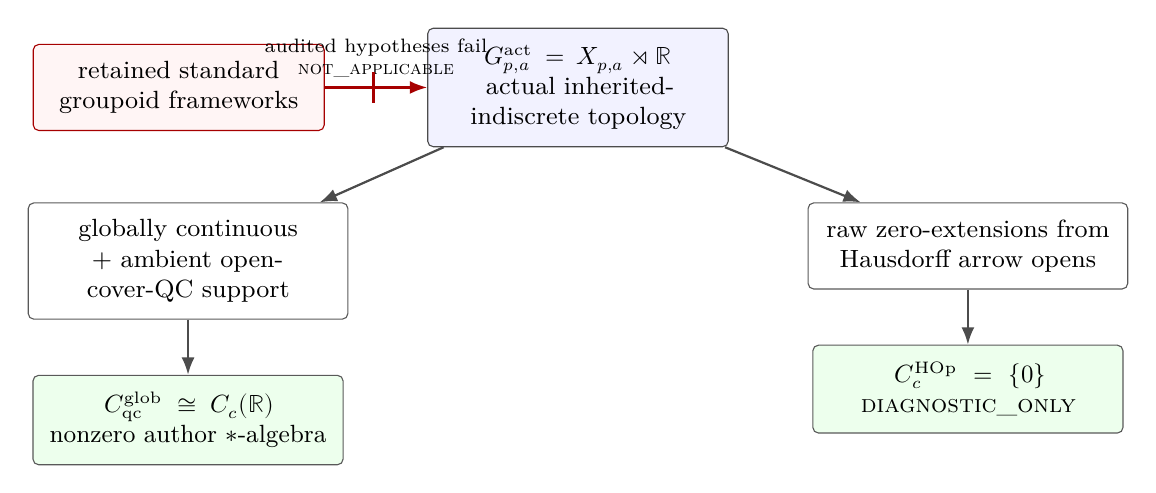
\begin{tikzpicture}[
  font=\small,
  node distance=7mm and 10mm,
  owner/.style={draw=black!70, rounded corners=2pt, fill=blue!5,
    align=center, inner sep=6pt, text width=0.28\textwidth},
  branch/.style={draw=black!65, rounded corners=2pt, align=center,
    inner sep=6pt, text width=0.30\textwidth},
  result/.style={draw=black!65, rounded corners=2pt, fill=green!7,
    align=center, inner sep=6pt, text width=0.29\textwidth},
  blocked/.style={draw=red!65!black, rounded corners=2pt, fill=red!4,
    align=center, inner sep=6pt, text width=0.27\textwidth},
  arr/.style={-{Latex[length=2.2mm]}, thick, draw=black!70},
  cross/.style={-{Latex[length=2.2mm]}, thick, draw=red!65!black}
]
\node[owner] (actual) {$G^{\mathrm{act}}_{p,a}=X_{p,a}\rtimes\mathbb R$\\
  actual inherited-indiscrete topology};

\node[branch, below left=of actual] (global) {globally continuous\\
  + ambient open-cover-QC support};
\node[branch, below right=of actual] (hopen) {raw zero-extensions from\\
  Hausdorff arrow opens};

\node[result, below=of global] (nonzero) {$C^{\mathrm{glob}}_{\mathrm{qc}}
  \cong C_c(\mathbb R)$\\nonzero author $*$-algebra};
\node[result, below=of hopen] (zero) {$C_c^{\mathrm{HOp}}=\{0\}$\\
  \textsc{diagnostic\_only}};

\node[blocked, left=13mm of actual] (frameworks) {retained standard\\
  groupoid frameworks};

\draw[arr] (actual) -- (global);
\draw[arr] (actual) -- (hopen);
\draw[arr] (global) -- (nonzero);
\draw[arr] (hopen) -- (zero);
\draw[cross] (frameworks.east) -- node[above, align=center, font=\scriptsize]
  {audited hypotheses fail\\\textsc{not\_applicable}} (actual.west);
\draw[red!65!black, line width=1.1pt]
  ($(frameworks.east)!0.48!(actual.west)+(0,2.0mm)$) --
  ($(frameworks.east)!0.48!(actual.west)+(0,-2.0mm)$);
\end{tikzpicture}
}
\caption{The convention split on the exact actual owner.  Global continuity
with ambient open-cover-quasi-compact support produces a nonzero author
$*$-algebra, whereas the raw Hausdorff-open span is zero and is
\Diag.  The crossed arrow records only that the retained frameworks' audited
hypotheses fail on this owner; it is not a universal nonexistence claim.}
\label{fig:convention-split}
\end{figure}

\noindent\textit{Prose equivalent for \cref{fig:convention-split}.}
Starting from the actual product $\Xpa\times\R$, one branch selects globally
continuous functions with quasi-compact ambient support and yields
$\Cglob\cong C_c(\R)$.  The other branch selects raw extensions from
Hausdorff arrow opens and yields zero.  Standard frameworks are not applied
because their stated actual-owner hypotheses fail.

\section{Source input, actual owner, and convention dictionary}
\label{sec:owners}

Fix a rational prime $p$ and a normalized companion-paper orbit label $a$.
Write $L_p=\log p$ and let $\Xpa$ be the corresponding inherited orbit.
Deninger's source owns the underlying right action and its stabilizer
$L_p\Z$; the companion theorem owns the actual nontrivial indiscrete
topology.  Paper 11 forms the transformation groupoid and owns the analytic
definitions below.  No ordinary-circle topology is imported into $\Xpa$.

It is useful to begin in a generic domain.  Let $X$ be a nonempty indiscrete
space and let
\[
  \alpha:X\times\R\longrightarrow X,\qquad (x,t)\longmapsto x\cdot t,
\]
be any right action of the additive group $\R$.  It is jointly continuous
because the codomain is indiscrete.  Set $G(X,\alpha)=X\times\R$ with the
product topology and the range-first operations
\begin{align}
 r(x,t)&=x, & s(x,t)&=x\cdot t,\label{eq:range-source}\\
 (x,t)(x\cdot t,u)&=(x,t+u), & (x,t)^{-1}&=(x\cdot t,-t).
 \label{eq:groupoid-operations}
\end{align}
No transitivity, freeness, period, or stabilizer is assumed in the generic
theorems.  The arithmetic specialization is $X=\Xpa$ and
$G(X,\alpha)=\Gact$.

Throughout, \emph{quasi-compact} means that every open cover has a finite
subcover.  It does not imply Hausdorffness.  For a function on $G$, support
means the closure of its nonzero set in the ambient product topology.

\begin{definition}[Three function owners]
The author global-QC space is
\[
 \Cglob(G)=\{f:G\to\C:f\text{ is continuous and }\supp_G(f)
 \text{ is quasi-compact}\}.
\]
When $X$ is nontrivial, the raw HOpen record is
\[
 \CHOp(G)=\operatorname{span}\{\widetilde h:
 U\subseteq G\text{ open Hausdorff},\ h\in C_c(U)\},
\]
where $\widetilde h$ is the raw zero-extension.  This record is a diagnostic
only.  Finally, $C_c(\Gstd)$ denotes the ordinary compactly supported
continuous functions on the standard Hausdorff proxy defined below.
\end{definition}

For each $x\in X$, let $G^x=r^{-1}(x)$ and
\[
 \rho_x:\R\to G^x,\qquad \rho_x(t)=(x,t),\qquad
 \lambda^x=(\rho_x)_*dt.
\]
The name \emph{GLOB-FIBRE-FAMILY} refers only to this author-defined family
and the properties proved in \cref{sec:convolution}.  Let
$\lambda_x=(\operatorname{inv})_*\lambda^x$ on $G_x=s^{-1}(x)$ and define
the author source-fibre operator $\Ind_x$ by the dense-domain formula in
\cref{sec:regular}.  The completion $\Cfull(G)$ is defined through the norm
transported from $C^*(\R)$ after the dense $*$-isomorphism is proved.
$\Cred(G)$ is defined through $\sup_x\|\Ind_x(\cdot)\|$.  These are not
denoted $C^*(G)$ or $C_r^*(G)$.

For the standard proxy, choose a set-level orbit chart
\[
 \theta:S_p^{\mathrm{std}}=\R/L_p\Z\longrightarrow\Xpa,
 \qquad \theta([r])=x^0\cdot r,
\]
with inverse $\beta$.  The circle $S_p^{\mathrm{std}}$ carries its ordinary
compact Hausdorff topology.  Put $\Gstd=S_p^{\mathrm{std}}\times\R$ with
the same right-action, range-first formulas and define
\begin{equation}
 J:\Gact\to\Gstd,\quad J(x,t)=(\beta(x),t),\qquad
 J^{-1}([r],t)=(\theta([r]),t).
 \label{eq:J}
\end{equation}
The function map, if well-defined, is contravariant:
\begin{equation}
 I(f)=f\circ J^{-1}.
 \label{eq:I}
\end{equation}
The directions in \cref{eq:J,eq:I} are part of the theorem, not a notational
choice.

\section{Arrow topology and factorization through time}
\label{sec:topology}

\begin{lemma}[Actual product topology]
\label{lem:topology}
The opens of $G=X\times\R$ are exactly $X\times U$ with $U$ open in
$\R$, and the closed sets are exactly $X\times F$ with $F$ closed.  For
every $A\subseteq G$,
\begin{equation}
 \overline A^{\,G}=X\times\overline{\pi_{\R}(A)}^{\,\R},
 \qquad \pi_{\R}(x,t)=t.
 \label{eq:closure}
\end{equation}
Every relative open subset of $K\subseteq G$ is
$K\cap\pi_{\R}^{-1}(U)$ for an open $U\subseteq\R$.
\end{lemma}

\begin{proof}
The only nonempty basic products are $X\times U$, and unions preserve this
form.  Complements give the closed sets.  A neighborhood of $(x,t)$ has the
form $X\times U$ with $t\in U$, so it meets $A$ exactly when $U$ meets
$\pi_{\R}(A)$.  This proves \cref{eq:closure}; intersecting ambient opens with
$K$ proves the relative statement.
\end{proof}

\begin{theorem}[Projection criterion for quasi-compactness]
\label{thm:qc}
For every $K\subseteq G$,
\begin{equation}
 K\text{ is quasi-compact}\quad\Longleftrightarrow\quad
 \pi_{\R}(K)\text{ is compact in }\R.
 \label{eq:qc}
\end{equation}
\end{theorem}

\begin{proof}
The continuous image of a quasi-compact space is quasi-compact, and in
Hausdorff $\R$ this is ordinary compactness.  Conversely, an open cover of
$K$ consists, after restriction, of sets
$K\cap\pi_{\R}^{-1}(U_i)$.  Their time projections cover the compact set
$\pi_{\R}(K)$, so finitely many suffice and the corresponding relative opens
cover $K$.
\end{proof}

The arrow space is second countable.  Each point has the quasi-compact
neighborhood $X\times[t-\varepsilon,t+\varepsilon]$ and a basis of open
neighborhoods with quasi-compact closure.  These positive local statements
do not imply local Hausdorffness.  If $X$ is nontrivial, $(x,t)$ and $(y,t)$
for $x\ne y$ have identical neighborhoods.  Hence $G$ is not $T_0$, no
nonempty arrow open is Hausdorff, and the space is nowhere locally
Hausdorff.  Moreover, no nonempty arrow open is quasi-compact: its nonempty
open time projection cannot be compact in the connected line.

\begin{proposition}[Topological groupoid]
\label{prop:topological-groupoid}
The operations in \cref{eq:range-source,eq:groupoid-operations} make $G$ a
topological groupoid.  The composable-pair chart
\[
 \Psi:X\times\R\times\R\longrightarrow G^{(2)},\qquad
 \Psi(x,t,u)=((x,t),(x\cdot t,u))
\]
is a homeomorphism.
\end{proposition}

\begin{proof}
The groupoid identities follow from the right-action law and addition.
Both the product subspace $G^{(2)}$ and $X\times\R^2$ have opens determined
only by $(t,u)$, making $\Psi$ and its inverse continuous.  Range and source
are continuous because their target is indiscrete.  In the chart,
multiplication is $(x,t,u)\mapsto(x,t+u)$, and inversion changes the time
coordinate by $t\mapsto-t$; both are continuous.  The unit map is continuous
for the same reason.
\end{proof}

\begin{theorem}[Continuous separated-target factorization]
\label{thm:t0-factor}
Let $Y$ be a $T_0$ space.  A map $F:G\to Y$ is continuous if and only if
there is a unique continuous $g:\R\to Y$ with
\begin{equation}
 F=g\circ\pi_{\R}.
 \label{eq:continuous-factor}
\end{equation}
\end{theorem}

\begin{proof}
Equal-time points are topologically indistinguishable.  A continuous map
into a $T_0$ target therefore takes the same value on each time fibre.
Choose $x_0\in X$ and set $g(t)=F(x_0,t)$.  The section
$t\mapsto(x_0,t)$ is continuous, hence so is $g$.  Conversely, the pullback
of a continuous $g$ by $\pi_{\R}$ is continuous, and surjectivity of the
projection gives uniqueness.
\end{proof}

The separation hypothesis is sharp.  A nonconstant map from a nontrivial
indiscrete $X$ into a nontrivial indiscrete target is continuous and may be
used at every time.  Thus the theorem does not classify arbitrary targets.

\begin{theorem}[Measurable factorization]
\label{thm:measurable-factor}
The topology-generated sigma-algebra is
\begin{equation}
 \Borel(G)=\{X\times B:B\in\Borel(\R)\}.
 \label{eq:borel}
\end{equation}
If $(Y,\Sigma_Y)$ is countably separated, a map
$F:(G,\Borel(G))\to(Y,\Sigma_Y)$ is measurable if and only if it factors
uniquely as $g\circ\pi_{\R}$ for a measurable $g$ on $\R$.
\end{theorem}

\begin{proof}
The displayed family is a sigma-algebra containing all opens.  Conversely,
the sets $B\subseteq\R$ for which $X\times B$ is Borel form a sigma-algebra
containing the time opens, proving \cref{eq:borel}.  Let $(E_n)$ be a
countable separating family in $Y$.  Each $F^{-1}(E_n)$ is $X\times B_n$,
so membership cannot distinguish two equal-time unit labels.  The separating
family forces $F$ to be constant on every time fibre.  A measurable section
then constructs $g$, and the converse and uniqueness are immediate.
\end{proof}

When $X$ is nontrivial, $(G,\Borel(G))$ is not countably separated even
though its sigma-algebra is countably generated.  No standard-Borel-source
claim is made.

\section{Global-QC functions and author fibre convolution}
\label{sec:convolution}

For $g:\R\to\C$, define
\[
 \Phi(g)(x,t)=g(t).
\]

\begin{theorem}[Exact global function classification]
\label{thm:phi}
The map
\[
 \Phi:C_c(\R)\longrightarrow\Cglob(G)
\]
is a linear bijection.  For every continuous $g$, with no support assumption,
\begin{equation}
 \supp_G\Phi(g)=X\times\supp_{\R}(g).
 \label{eq:support}
\end{equation}
\end{theorem}

\begin{proof}
Apply \cref{thm:t0-factor} to the Hausdorff target $\C$.  This classifies all
globally continuous functions as unique time pullbacks.  Their nonzero
locus is $X\times\{t:g(t)\ne0\}$, and \cref{eq:closure} gives
\cref{eq:support}.  By \cref{thm:qc}, the ambient support is quasi-compact
exactly when $\supp_{\R}(g)$ is compact.  Both directions of the support gate
are therefore explicit.
\end{proof}

\begin{theorem}[Author range-fibre contract]
\label{thm:fibres}
For each $x\in X$, $\rho_x$ is a homeomorphism $\R\to G^x$ and $\lambda^x$
is a positive full-support Radon measure on that locally compact Hausdorff
fibre.  If $f=\Phi(g)\in\Cglob(G)$, then
\begin{equation}
 \int_{G^x}f\,d\lambda^x=\int_{\R} g(t)\,dt,
 \label{eq:fibre-integral}
\end{equation}
which is absolutely finite and independent of $x$.  The family also
satisfies left invariance on the named function domain.
\end{theorem}

\begin{proof}
The subspace opens of $G^x=\{x\}\times\R$ are exactly
$\{x\}\times U$, so the first assertion is transport from Lebesgue measure.
The compact time support of $g$ proves absolute integrability and
\cref{eq:fibre-integral}.  If $\gamma=(x,t)$ and
$\eta=(x\cdot t,u)\in G^{s(\gamma)}$, then
$\gamma\eta=(x,t+u)$; translation invariance gives
\[
 \int_{G^{s(\gamma)}} f(\gamma\eta)\,d\lambda^{s(\gamma)}(\eta)
 =\int_{\R} g(t+u)\,du
 =\int_{\R} g(v)\,dv.
\]
\end{proof}

This verifies the GLOB-FIBRE-FAMILY contract directly.  It does not invoke a
retained Haar-system theorem on the actual owner.

For $f,h\in\Cglob(G)$ define, using the range-first coordinates,
\begin{align}
 (f*h)(x,t)&=\int_{\R} f(x,u)h(x\cdot u,t-u)\,du,\label{eq:arrow-convolution}\\
 f^*(x,t)&=\overline{f(x\cdot t,-t)}.\label{eq:arrow-involution}
\end{align}

\begin{theorem}[Global-QC convolution $*$-algebra]
\label{thm:star-algebra}
For $g,k\in C_c(\R)$ put
\[
 (g*k)(t)=\int_{\R} g(u)k(t-u)\,du,
 \qquad g^{\sharp}(t)=\overline{g(-t)}.
\]
Then
\begin{equation}
 \Phi(g)*\Phi(k)=\Phi(g*k),\qquad
 \Phi(g)^*=\Phi(g^{\sharp}),
 \label{eq:intertwining}
\end{equation}
and $\Phi$ is a $*$-isomorphism from the ordinary compactly supported group
convolution algebra onto $\Cglob(G)$.
\end{theorem}

\begin{proof}
Substitution in \cref{eq:arrow-convolution} gives
\[
 (\Phi(g)*\Phi(k))(x,t)
 =\int_{\R} g(u)k(t-u)\,du.
\]
The integrand is supported on
$\supp(g)\cap(t-\supp(k))$, so it is absolutely integrable.  Uniform
continuity of a compactly supported continuous function yields
\[
 |(g*k)(t+h)-(g*k)(t)|
 \le \|g\|_1\sup_v|k(v+h)-k(v)|\longrightarrow0.
\]
Also $\supp(g*k)\subseteq\supp(g)+\supp(k)$, a compact set.  The inverse
formula gives the second identity in \cref{eq:intertwining}, with
$\supp(g^{\sharp})=-\supp(g)$.

For associativity, the absolute-integrability estimate
\[
 \iint_{\R^2}|g(u)k(v-u)\ell(t-v)|\,du\,dv
 \le \|\ell\|_{\infty}\|g\|_1\|k\|_1
\]
licenses Fubini and the substitution $w=v-u$.  This proves
$(g*k)*\ell=g*(k*\ell)$.  Conjugation under the integral and reflection
give $(g*k)^{\sharp}=k^{\sharp}*g^{\sharp}$ and
$(g^{\sharp})^{\sharp}=g$.  Transport through the bijection in
\cref{thm:phi} completes the proof.
\end{proof}

The action has disappeared from \cref{eq:intertwining} as a conclusion of
the global factorization theorem.  We did not assume that the transformation
groupoid was the group $\R$.

\section{Unit-regular operators and transported completions}
\label{sec:regular}

The exact source fibre is
\begin{equation}
 G_x=\{(x\cdot(-t),t):t\in\R\},\qquad
 \vartheta_x(t)=(x\cdot(-t),t).
 \label{eq:source-fibre}
\end{equation}
It has the subspace topology transported from $\R$.  Inversion sends
$(x,v)$ to $\vartheta_x(-v)$, so reflection invariance of Lebesgue measure
gives
\begin{equation}
 \lambda_x=(\operatorname{inv})_*\lambda^x=(\vartheta_x)_*dt.
 \label{eq:source-measure}
\end{equation}
Consequently
\begin{equation}
 U_x:L^2(G_x,\lambda_x)\to L^2(\R),\qquad
 (U_x\xi)(t)=\xi(\vartheta_x(t))
 \label{eq:Ux}
\end{equation}
is unitary.

\begin{theorem}[Dense-domain kernel and bounded extension]
\label{thm:regular}
For $f=\Phi(g)$ and initially $\xi\in C_c(G_x)$, set
\begin{equation}
 [\Ind_x(f)\xi](\gamma)=
 \int_{G_x}f(\gamma\eta^{-1})\xi(\eta)\,d\lambda_x(\eta).
 \label{eq:Ind}
\end{equation}
The integral is pointwise absolutely finite on this dense domain and extends
uniquely to a bounded operator on $L^2(G_x,\lambda_x)$.  Under \cref{eq:Ux},
\begin{equation}
 [U_x\Ind_x(\Phi(g))U_x^{-1}\zeta](t)
 =\int_{\R} g(t-u)\zeta(u)\,du
 =[\lambda_{\R}(g)\zeta](t),
 \label{eq:regular-kernel}
\end{equation}
and $\|\Ind_x(\Phi(g))\|\le\|g\|_1$.
\end{theorem}

\begin{proof}
Write $\gamma=\vartheta_x(t)$ and $\eta=\vartheta_x(u)$.  Then
$\eta^{-1}=(x,-u)$ and the range-first product is
\[
 \gamma\eta^{-1}=(x\cdot(-t),t-u).
\]
This proves the sign $g(t-u)$ in \cref{eq:regular-kernel}.  On compactly
supported vectors, the integrand is bounded on compact support and hence
absolutely integrable.  Young's inequality follows from Minkowski and
translation invariance:
\[
 \|\lambda_{\R}(g)\zeta\|_2
 \le\int_{\R}|g(v)|\,\|\zeta(\,\cdot-v)\|_2\,dv
 =\|g\|_1\|\zeta\|_2.
\]
Density gives the unique bounded extension.  For arbitrary $L^2$ vectors,
the equality is an $L^2$ identity, not a claim that every equivalence-class
representative has a pointwise integral everywhere.
\end{proof}

\begin{proposition}[Regular $*$-representation]
\label{prop:regular-star}
Each $\Ind_x$ is an author-defined bounded $*$-representation:
\[
 \Ind_x(f*h)=\Ind_x(f)\Ind_x(h),\qquad
 \Ind_x(f^*)=\Ind_x(f)^*.
\]
Moreover, $\lambda_{\R}$ is faithful on $C_c(\R)$.
\end{proposition}

\begin{proof}
Associativity on $C_c(\R)$ gives multiplicativity on the dense vector domain
and boundedness extends the identity.  With the inner product linear in the
first variable, absolute Fubini and a change of variables give
$\lambda_{\R}(g)^*=\lambda_{\R}(g^{\sharp})$.  For faithfulness, if $g\ne0$ take
$\zeta(u)=\overline{g(-u)}$.  Then
\[
 [\lambda_{\R}(g)\zeta](0)=\int_{\R}|g(-u)|^2\,du>0.
\]
The convolution is continuous, so it represents a nonzero $L^2$ class.
\end{proof}

\begin{corollary}[Author reduced norm]
\label{cor:reduced}
For every nonempty $X$ and every $g\in C_c(\R)$,
\begin{equation}
 \|\Phi(g)\|_{\mathrm{red,glob}}
 :=\sup_{x\in X}\|\Ind_x(\Phi(g))\|
 =\|\lambda_{\R}(g)\|.
 \label{eq:rednorm}
\end{equation}
This is a norm.
\end{corollary}

All base units have the same kernel and norm.  This conclusion was obtained
from the exact source fibre and the inversion-pushed measure, not from a
standard actual-groupoid regular-representation theorem.

Define the full norm separately by
\begin{equation}
 \|\Phi(g)\|_{\mathrm{full,glob}}:=\|g\|_{C^*(\R)}.
 \label{eq:fullnorm}
\end{equation}

\begin{theorem}[Transported completions]
\label{thm:completions}
Completion of the two named norms gives author-defined $*$-isomorphisms
\begin{equation}
 \Cfull(G)\cong C^*(\R),\qquad
 \Cred(G)\cong C_r^*(\R).
 \label{eq:transport}
\end{equation}
Because $\R$ is abelian and amenable, the group full and reduced norms agree.
With
\[
 \widehat g(\xi)=\int_{\R} g(t)e^{-it\xi}\,dt,
\]
the group Fourier theorem yields
\begin{equation}
 \Cfull(G)\cong\Cred(G)\cong C_0(\R).
 \label{eq:Fourier-model}
\end{equation}
\end{theorem}

\begin{proof}
The first line is definitional for the full norm and follows from
\cref{eq:rednorm} for the reduced norm.  Williams identifies the left-regular
group norm, proves the LCA Fourier model, and records the abelian/amenable
full--reduced equality \cite[Example~1.80, Proposition~3.1, Examples~7.9
and 7.11, and Theorem~7.13]{Williams2007}.  These theorems belong to the
group $\R$ and apply only after \cref{eq:transport} has been established.
\end{proof}

The definitions in \cref{eq:rednorm,eq:fullnorm} are different even though
their completions have isomorphic final models.  Equality is credited to
amenability of the group $\R$, not to amenability of the actual groupoid.

\section{Hausdorff-open diagnostic and strict standard proxy}
\label{sec:proxy}

\begin{proposition}[Raw HOpen diagnostic]
\label{prop:hopen}
If $X$ is nontrivial indiscrete, no nonempty open subset of $G$ is Hausdorff
and
\begin{equation}
 \CHOp(G)=\{0\}.
 \label{eq:hopen-zero}
\end{equation}
\end{proposition}

\begin{proof}
A nonempty open is $X\times U$.  Choose $t\in U$ and distinct $x,y\in X$.
The equal-time points $(x,t)$ and $(y,t)$ have identical relative
neighborhoods, so the open is not even $T_0$.  Thus the empty patch is the
only Hausdorff open and contributes only the zero extension.
\end{proof}

The zero in \cref{eq:hopen-zero} is \Diag.  It has no licensed convolution,
norm, completion, or standard-algebra status.  If $g\in C_c(\R)$ is nonzero,
$\Phi(g)$ is an explicit nonzero element of $\Cglob(G)$ on the same topology.
The two records therefore form a genuine convention split.

\begin{table}[htbp]
\centering\small
\caption{Framework applicability and owner boundary.  The table compares
the audited hypotheses of the retained sources; it makes no universal claim
about every possible non-Hausdorff convolution theory.}
\label{tab:framework-applicability}
\begin{tabularx}{\textwidth}{P{0.19\textwidth}P{0.30\textwidth}P{0.20\textwidth}Y}
\toprule
Record & Audited actual-owner obstruction & Classification & Licensed role \\
\midrule
Tu \cite{Tu2004} & Tu-local compactness requires compact Hausdorff neighborhoods and hence local Hausdorffness & \NA & terminology and raw HOpen comparator \\
Muhly--Williams \cite{MuhlyWilliams2008} & Hausdorff units and compact Hausdorff arrow neighborhoods fail & \NA & accepted raw patch-span practice only \\
Exel \cite{Exel2011} & unit is non-Hausdorff and continuous-$\R$ range/source are not etale & \NA & independent boundary only \\
Buss--Holkar--Meyer \cite{BussHolkarMeyer2018} & Hausdorff groupoid standing hypothesis fails & \NA & full proxy bridge only \\
$\CHOp(G)$ & direct author raw diagnostic & \Diag & exact value $0$, no algebraic promotion \\
GLOB-FIBRE-FAMILY, $\Ind_x$ & direct author definitions with proved contracts & \textsc{author\_defined\_\allowbreak direct} & actual global domain only \\
Group $\R$ & ordinary LCA harmonic analysis & \textsc{applicable\_\allowbreak group\_R} & transport after direct dense/norm proofs \\
Standard proxy & ordinary compact Hausdorff circle and arrow space & \textsc{applicable\_\allowbreak proxy\_only} & full crossed-product and comparison records \\
\bottomrule
\end{tabularx}
\end{table}

The table proves non-applicability of named sources, not nonexistence of every
conceivable theory.  The direct global-QC construction itself demonstrates
why the latter statement would be false.

\begin{theorem}[One-sided actual/proxy topology]
\label{thm:J}
The map $J$ in \cref{eq:J} is a set-groupoid isomorphism.  Its topology
direction is strict:
\begin{equation}
 J\text{ is not continuous},\qquad J^{-1}\text{ is continuous}.
 \label{eq:J-direction}
\end{equation}
\end{theorem}

\begin{proof}
Equivariance $\beta(x\cdot t)=\beta(x)+t$ verifies source and product:
\[
 J((x,t)(x\cdot t,u))=(\beta(x),t+u)
 =J(x,t)J(x\cdot t,u),
\]
and inverse and units follow similarly.  Every actual arrow open is
$X\times U$, whose inverse image under $J^{-1}$ is
$S_p^{\mathrm{std}}\times U$, proving continuity of $J^{-1}$.  If $V$ is
a nonempty proper open circle arc, then $V\times\R$ is proxy-open but its
inverse image under $J$ is $\beta^{-1}(V)\times\R$, a nonempty proper
unit-coordinate subset and therefore not actual-open.
\end{proof}

\begin{theorem}[Strict test-function map]
\label{thm:I}
The map
\[
 I:\Cglob(\Gact)\longrightarrow C_c(\Gstd),\qquad I(f)=f\circ J^{-1},
\]
is an injective $*$-homomorphism at the test-function level.  It preserves
the range-fibre Lebesgue measures, fibre integrals, support, convolution, and
involution.  Its exact image is
\begin{equation}
 \Aconst=\{F\in C_c(\Gstd):F([r],t)=F([s],t)
 \text{ for all }[r],[s],t\},
 \label{eq:Aconst}
\end{equation}
and $\Aconst$ is a proper subalgebra.
\end{theorem}

\begin{proof}
If $f=\Phi(g)$, then
\[
 I(f)([r],t)=g(t),\qquad
 \supp_{\mathrm{std}}I(f)=S_p^{\mathrm{std}}\times\supp_{\R}(g),
\]
which is compact.  Surjectivity of $J^{-1}$ gives injectivity.  On each range
fibre, $J$ preserves the time coordinate and hence the pushed-forward
Lebesgue measure.  The proxy operations are
\begin{align*}
 (F*_{\mathrm{std}}H)([r],t)
 &=\int_{\R} F([r],u)H([r+u],t-u)\,du,\\
 F^*([r],t)&=\overline{F([r+t],-t)},
\end{align*}
so unit-constant functions reproduce the formulas in
\cref{eq:intertwining}.

Every image lies in $\Aconst$.  Conversely, if $F$ lies in $\Aconst$, set
$g(t)=F([r_0],t)$.  Compactness of $\supp(F)$ projects to compactness of
$\supp(g)$, and $F=I(\Phi(g))$.  Finally, for nonzero $k\in C_c(\R)$,
\begin{equation}
 F_{\mathrm{out}}([r],t)=e^{2\pi i r/L_p}k(t)
 \label{eq:strict-witness}
\end{equation}
is continuous and compactly supported on the proxy but varies with $[r]$.
Thus it is not in $\Aconst$.
\end{proof}

\paragraph{Completion stop.}
Theorem~\ref{thm:I} gives no map between any completions.  Such a map would
require a named target norm and an independent boundedness or isometry proof.
The proxy source ladder does not provide this missing estimate.  BHM gives a
full transformation-groupoid/full crossed-product bridge
\cite[Theorem~7.1]{BussHolkarMeyer2018}; Green and MRW give full-level Morita
equivalence \cite[Proposition~3, physical p.~13 / printed p.~203]{Green1978}
\cite[Theorem~2.8, physical p.~8 / printed p.~10]{MuhlyRenaultWilliams1987}; Brown--Green--Rieffel
gives stable isomorphism under its hypotheses
\cite[Theorem~1.2, physical p.~4 / printed p.~351]{BrownGreenRieffel1977};
and Williams gives a separate unstabilized full homogeneous-space tensor
model \cite[Eq.~(4.63) and Theorem~4.30]{Williams2007}.  These strengths are
not interchangeable and remain proxy-only.  In particular, none proves
boundedness, density, Morita equivalence, stable isomorphism, or a completion
extension of $I$.

\begin{figure}[htbp]
\centering
\resizebox{0.99\textwidth}{!}{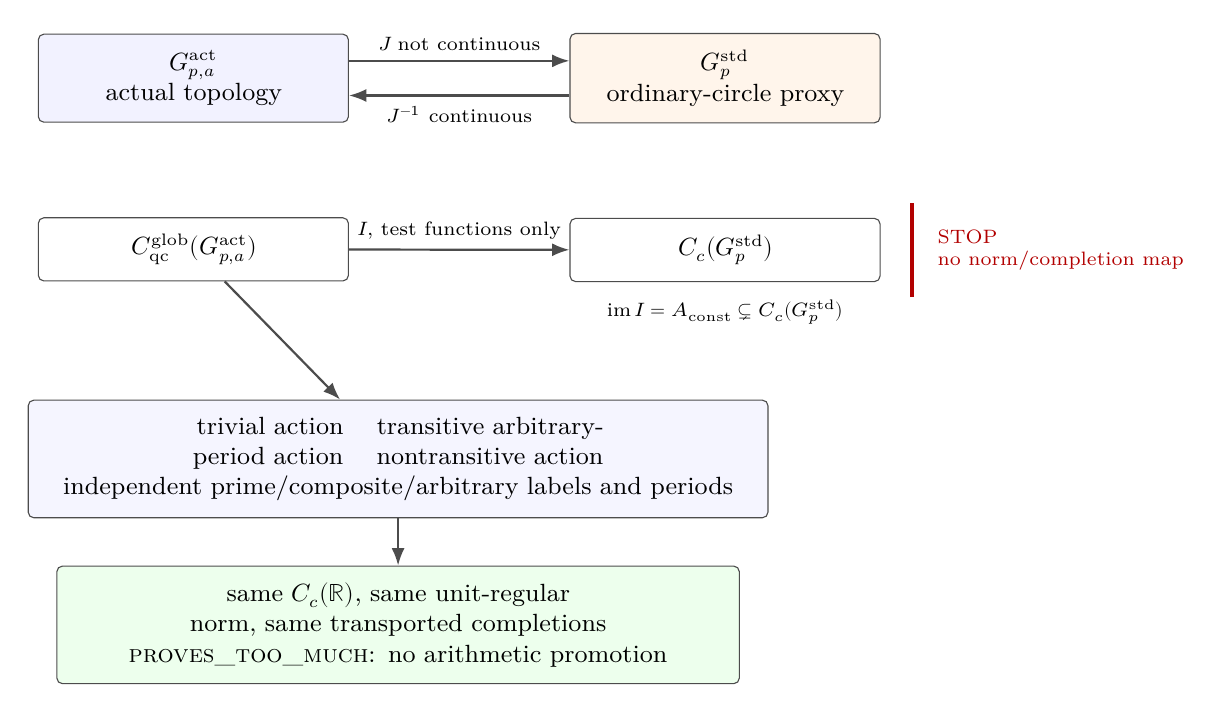
\begin{tikzpicture}[
  font=\small,
  node distance=6mm and 9mm,
  box/.style={draw=black!70, rounded corners=2pt, align=center,
    inner sep=6pt, text width=0.29\textwidth},
  wide/.style={draw=black!70, rounded corners=2pt, fill=blue!4,
    align=center, inner sep=6pt, text width=0.74\textwidth},
  result/.style={draw=black!70, rounded corners=2pt, fill=green!7,
    align=center, inner sep=6pt, text width=0.68\textwidth},
  arr/.style={-{Latex[length=2.2mm]}, thick, draw=black!70},
  stop/.style={line width=1.5pt, draw=red!70!black}
]
\node[box, fill=blue!5] (act) {$G^{\mathrm{act}}_{p,a}$\\actual topology};
\node[box, fill=orange!8, right=28mm of act] (std) {$G^{\mathrm{std}}_p$\\
  ordinary-circle proxy};
\draw[arr] ($(act.east)+(0,2.2mm)$) --
  node[above, font=\scriptsize] {$J$ not continuous} ($(std.west)+(0,2.2mm)$);
\draw[arr] ($(std.west)+(0,-2.2mm)$) --
  node[below, font=\scriptsize] {$J^{-1}$ continuous} ($(act.east)+(0,-2.2mm)$);

\node[box, below=12mm of act] (alg) {$C^{\mathrm{glob}}_{\mathrm{qc}}
  (G^{\mathrm{act}}_{p,a})$};
\node[box, below=12mm of std] (proxyalg) {$C_c(G^{\mathrm{std}}_p)$};
\draw[arr] (alg) -- node[above, font=\scriptsize] {$I$, test functions only}
  (proxyalg);
\node[font=\scriptsize, below=1mm of proxyalg] (image)
  {$\operatorname{im}I=A_{\mathrm{const}}\subsetneq C_c(G^{\mathrm{std}}_p)$};
\draw[stop] ($(proxyalg.east)+(4mm,-6mm)$) -- ($(proxyalg.east)+(4mm,6mm)$);
\node[anchor=west, text=red!70!black, font=\scriptsize, align=left]
  at ($(proxyalg.east)+(6mm,0)$) {STOP\\no norm/completion map};

\node[wide, below=15mm of alg, xshift=26mm] (controls)
  {trivial action \quad transitive arbitrary-period action \quad
   nontransitive action\\independent prime/composite/arbitrary labels and periods};
\node[result, below=of controls] (collapse)
  {same $C_c(\mathbb R)$, same unit-regular norm, same transported completions\\
   \textsc{proves\_too\_much}: no arithmetic promotion};
\draw[arr] (alg) -- (controls);
\draw[arr] (controls) -- (collapse);
\end{tikzpicture}
}
\caption{The one-sided proxy comparison and the action-blind obstruction.
The hard stop after $C_c(\Gstd)$ indicates that $I$ is proved only on test
functions and has the proper image $\Aconst$; no completion arrow is defined.
The lower branch records that distinct action, orbit, label, and period
controls yield the same global analytic records, preventing arithmetic
promotion.}
\label{fig:proxy-action-blind}
\end{figure}

\noindent\textit{Prose equivalent for \cref{fig:proxy-action-blind}.}
The actual and proxy groupoids are set-groupoid isomorphic, but continuity
holds only from the proxy to the actual topology.  Pullback gives a strict
test-function inclusion whose image is unit-constant, and the comparison
stops before norms.  Independently, trivial, transitive, nontransitive, and
label-period controls all collapse to the same group-$\R$ algebra and norm.

\section{Action blindness, controls, and Route consequences}
\label{sec:controls-route}

\begin{theorem}[Generic action-blind theorem]
\label{thm:action-blind}
Let $X$ be any nonempty indiscrete space and let $\alpha$ be any right
$\R$-action.  Then
\begin{enumerate}
\item $\Phi_X:C_c(\R)\to\Cglob(G(X,\alpha))$ is a canonical
  $*$-isomorphism;
\item the author range-fibre integrals, convolution, and involution are
  independent of $X$ and $\alpha$ under $\Phi_X$;
\item every author unit-regular operator is unitarily $\lambda_{\R}$;
\item the author reduced and transported full norms are the ordinary group
  norms, and their completions are the group-$\R$ models in
  \cref{eq:Fourier-model}.
\end{enumerate}
If $X$ is nontrivial, $\CHOp(G(X,\alpha))=0$.  If $X$ is a singleton, the
global convolution conclusion remains true but the HOpen-zero statement
does not: the singleton product is Hausdorff.
\end{theorem}

\begin{proof}
The topology, factorization, and support arguments in
\cref{lem:topology,thm:qc,thm:t0-factor,thm:phi} do not mention the action.
For $f=\Phi_X(g)$ and $h=\Phi_X(k)$,
\[
 (f*h)(x,t)=\int g(u)k(t-u)\,du,
 \qquad f^*(x,t)=\overline{g(-t)},
\]
so the action disappears from the operations.  The range-fibre formula is
ordinary Lebesgue integration.  The source chart
$\vartheta_x(t)=(x\cdot(-t),t)$ and the computation
$\vartheta_x(t)\vartheta_x(u)^{-1}=(x\cdot(-t),t-u)$ give the same regular
kernel at every unit.  The norm and completion statements follow exactly as
in \cref{sec:regular}.  For nontrivial $X$, \cref{prop:hopen} is independent
of the action.  The singleton exception is immediate.
\end{proof}

\begin{corollary}[Adversarial mathematical controls]
\label{cor:math-controls}
The conclusion of \cref{thm:action-blind} is unchanged for:
\begin{enumerate}
\item a nontrivial indiscrete $X$ with the trivial action, whose stabilizers
  are all of $\R$;
\item $X=(\{0,1\}\times\R/\Z)_{\mathrm{indisc}}$ with two nontransitive
  circle orbits and stabilizer $\Z$;
\item $X_{\ell,L}=(\{\ell\}\times\R/L\Z)_{\mathrm{indisc}}$ with arbitrary
  $L>0$ and a transitive action;
\item independent prime, composite, or arbitrary labels and independent
  positive periods.
\end{enumerate}
\end{corollary}

The nontransitive control is deliberately infinite.  Since $\R$ is
divisible, it has no nontrivial finite quotient, so a nontrivial action of
$\R$ on a finite set would be a false control.  The exact controls show that
the theorem proves too much for arithmetic specificity: different orbit
decompositions and stabilizers yield the same analytic signature.

\begin{corollary}[Rational-Witt fixed-orbit application]
\label{cor:rational-witt}
For every rational prime $p$ and every normalized companion-paper orbit label
$a$, the actual fixed-orbit groupoid $\Gact$ satisfies
\[
 \Cglob(\Gact)\cong C_c(\R),\qquad
 \CHOp(\Gact)=0,
\]
and its author unit-regular norms and transported completions are the group
$\R$ records of \cref{eq:rednorm,eq:Fourier-model}.  The analytic output
retains none of $p$, $a$, $L_p$, the action, the orbit decomposition, or the
stabilizer $L_p\Z$.
\end{corollary}

The host-versus-analytic distinction is essential.  The concrete groupoid
still has $\Xpa$, its source and range maps, right action, and stabilizer as
relations.  The corollary states only that these data vanish after passage to
the named function, operator, norm, and completion records.  It is fixed-
orbit only and supplies no prime-coproduct, packet, or full-suspension theorem.

\subsection{Deterministic reproducibility receipt}

The direct proofs above establish the universal continuous statements.  A
standard-library-only Python package supplies finite regression oracles and
adversarial witnesses.  Its frozen manifest has SHA-256
\texttt{de55c58ad7efc133b0d0865f392a30b52f6b05f89f64878cea0910b7eab557ea}.
The exact receipt is:
\begin{itemize}
\item 57/57 unit tests passed;
\item 12 CSV artifacts containing 642 data rows;
\item 5/5 intentional source/range and sign negatives detected;
\item strict verify-only passed for checked-in results and for two fresh
  generations;
\item all 13 generated artifacts were byte-identical across checked-in,
  fresh-one, and fresh-two runs;
\item the forbidden Python cache/bytecode scan passed.
\end{itemize}
The suite includes topology enumeration, $T_0$ and measurable target
factorization, support projection, convolution and involution, unit-regular
matrices, HOpen zero, proxy strictness, action blindness, and independent
label-period changes.  It uses no network, external package, external
dataset, randomness, fitted parameter, target-zero table, or timestamp.
These finite checks are witnesses and regression guards.  They do not prove
the universal topological or analytic theorems.

\subsection{Typed Route ledger}

Seven Stage-11 records evaluate seven nonconflated owners.  The concrete
actual algebra and HOpen diagnostic retain only a weak host relation.  The
test map has a weak relation with evidence status \textsc{modeling\_choice}.
The abstract algebra, transported completions, and generic control have
already erased their arithmetic host.  Every record fails A1 through A4;
every A2--A4 failure is \textsc{not\_testable}, because the same owner has no
determinant, global analytic object, or natural lift.

\begin{table}[htbp]
\centering\scriptsize
\caption{Stage-11 Route summary; the complete hashes and tuple strings are
transcribed without abbreviation in the adjacent ordered ledgers.  The three
exploratory rows are scoped negative structural priors, not weak positive
arithmetic results.  All rows have
\texttt{route\_b\_invocation\_allowed: false}.}
\label{tab:route-ledger}
\begin{tabularx}{\textwidth}{P{0.20\textwidth}P{0.22\textwidth}P{0.34\textwidth}Y}
\toprule
Candidate & SHA-256 & $(A0,A1,A2,A3,A4)$ & Overall \\
\midrule
\texttt{DEN-EF-ACTUAL-GLOB-QC-CONV-P} & \texttt{ce52ba0f...e551} & $(\mathrm{WEAK},\mathrm{FAIL},\mathrm{FAIL},\mathrm{FAIL},\mathrm{FAIL})$ & exploratory \\
\texttt{DEN-EF-GLOB-QC-ABSTRACT-CCR} & \texttt{775fb3ac...6ccd} & $(\mathrm{FAIL},\mathrm{FAIL},\mathrm{FAIL},\mathrm{FAIL},\mathrm{FAIL})$ & rejected \\
\texttt{DEN-EF-GLOB-FULL-TRANSPORT-R} & \texttt{fb1f8bf7...8830} & $(\mathrm{FAIL},\mathrm{FAIL},\mathrm{FAIL},\mathrm{FAIL},\mathrm{FAIL})$ & rejected \\
\texttt{DEN-EF-GLOB-RED-REGULAR-R} & \texttt{45887d09...24b5} & $(\mathrm{FAIL},\mathrm{FAIL},\mathrm{FAIL},\mathrm{FAIL},\mathrm{FAIL})$ & rejected \\
\texttt{DEN-EF-ACTUAL-HOPEN-DIAGNOSTIC-P} & \texttt{25908c99...c6d7} & $(\mathrm{WEAK},\mathrm{FAIL},\mathrm{FAIL},\mathrm{FAIL},\mathrm{FAIL})$ & exploratory \\
\texttt{DEN-EF-ACTUAL-STD-TEST-MAP-P} & \texttt{e904f85d...cfac} & $(\mathrm{WEAK},\mathrm{FAIL},\mathrm{FAIL},\mathrm{FAIL},\mathrm{FAIL})$ & exploratory \\
\texttt{INDISC-R-ACTION-GLOB-CONV-CONTROL} & \texttt{23480710...a1b} & $(\mathrm{FAIL},\mathrm{FAIL},\mathrm{FAIL},\mathrm{FAIL},\mathrm{FAIL})$ & rejected \\
\bottomrule
\end{tabularx}
\end{table}

The abbreviated hashes in \cref{tab:route-ledger} correspond, in order, to
the full SHA-256 values
\begin{align*}
&\texttt{ce52ba0fddf39652a37992ff7babeb590bfcb5ce8853ee6aa87b2c877634e551},\\
&\texttt{775fb3ac86771744d3f15f708a73fc634992f770a8d7b3d04f570563054a6ccd},\\
&\texttt{fb1f8bf736099a2eca5175d818ad7a00f7f1de2d0ddb699135e035ab311d8830},\\
&\texttt{45887d091bb97853febaf0329e7035655e69ec44c49ee7919ce55a8ef3de24b5},\\
&\texttt{25908c995d5a1f2a6f8478d62715e7cf4fc653b76ae2f6bf9fdfe71f8cc3c6d7},\\
&\texttt{e904f85d078e84188f6d40a07e3e1fb1c7426068b8c4a9c4a773df221fd2cfac},\\
&\texttt{23480710707367d9f77b4896a7c85e073b17dcc5a4f8aae3814bff972d27ba1b}.
\end{align*}
The corresponding tuples, again in table order and transcribed without
abbreviation, are:
\begin{enumerate}[leftmargin=2.5em]
\item \texttt{(A0\_WEAK\_ARITHMETIC\_RELATION,}\newline
  \texttt{A1\_FAIL,A2\_FAIL,A3\_FAIL,A4\_FAIL)};
\item \texttt{(A0\_FAIL,A1\_FAIL,A2\_FAIL,A3\_FAIL,A4\_FAIL)};
\item \texttt{(A0\_FAIL,A1\_FAIL,A2\_FAIL,A3\_FAIL,A4\_FAIL)};
\item \texttt{(A0\_FAIL,A1\_FAIL,A2\_FAIL,A3\_FAIL,A4\_FAIL)};
\item \texttt{(A0\_WEAK\_ARITHMETIC\_RELATION,}\newline
  \texttt{A1\_FAIL,A2\_FAIL,A3\_FAIL,A4\_FAIL)};
\item \texttt{(A0\_WEAK\_ARITHMETIC\_RELATION,}\newline
  \texttt{A1\_FAIL,A2\_FAIL,A3\_FAIL,A4\_FAIL)};
\item \texttt{(A0\_FAIL,A1\_FAIL,A2\_FAIL,A3\_FAIL,A4\_FAIL)}.
\end{enumerate}
Exactly three rows are exploratory negative priors and four are rejected.
No A-coordinate is borrowed from another owner.  An abstract bounded
convolution representation on $L^2(\R)$ is not a Hilbert--Polya operator,
and every record has $A4\_\mathrm{FAIL}$.  Hence Route B is false and no
Route-B record exists.

\section{Limitations and conclusion}
\label{sec:conclusion}

This paper establishes an exact theorem plus an obstruction.  On every
hash-locked rational-Witt fixed orbit with its actual inherited topology,
the author global-QC convention gives a nonzero convolution $*$-algebra
canonically isomorphic to $C_c(\R)$.  The author source-fibre family is
unitarily the left regular group representation, and the separately defined
transported completions identify with $C_0(\R)$.  Under the raw
Hausdorff-open convention, however, the diagnostic span is zero.  The
ordinary-circle proxy supplies more test functions, but the actual image is
only the proper unit-coordinate-constant subalgebra and the proof stops
before every norm comparison.

Several limitations are structural rather than technical.  First, the
framework audit is finite: it establishes that the retained Tu,
Muhly--Williams, Exel, and BHM actual-owner hypotheses fail.  It does not
prove that no other non-Hausdorff convolution framework could be developed.
Second, GLOB-FIBRE-FAMILY, $\Ind_x$, $\Cfull$, and $\Cred$ are explicit
author records.  Their direct proofs do not turn them into standard
actual-groupoid objects.  Third, the comparison with the standard proxy is
test-level only.  Nothing here proves density, boundedness, an isometry,
Morita equivalence, stable isomorphism, or a completion extension of $I$.
Fourth, the result is fixed-orbit only.  No packet aggregation, prime
coproduct, full suspension, determinant, functional equation, explicit
formula, quantization, or Route-B entry is constructed.

The novelty assessment is likewise bounded.  As of 2026-08-15, the
documented bounded Phase-2 search located no precedent for the exact
rational-Witt actual-orbit convention-split package.  This sentence reports
only the documented search.  The generic indiscrete-product theorem, group
convolution on $\R$, the HOpen literature, and standard transformation-
groupoid theory receive no individual priority claim.

Most importantly, the generic theorem separates the host from its analytic
shadow.  The host still contains the rational-Witt action, orbit, and
stabilizer.  Global separated-valued continuity removes the unit coordinate,
after which convolution, regular operators, and transported norms cannot
recover it.  The same result on trivial and nontransitive actions is not a
defect in the proof; it is the decisive evidence that the collapsed analytic
object is unsuitable for arithmetic promotion.

Any successor owner should therefore meet three minimum conditions before
receiving arithmetic credit.  It should be source-canonical rather than a
retopologized modeling choice, it should retain enough action data to survive
its analytic functor, and it should distinguish the rational-Witt action from
at least one trivial or nontransitive control.  An enriched local, sheaf, or
stack construction may be investigated only after a fresh source, owner, and
domain lock; none is asserted to work here.  In particular, the actual host,
the erased group-$\R$ completion, and the standard proxy may not be spliced
together to manufacture a positive result.

\section*{Declarations}

\paragraph{Author contributions.}
Final CRediT roles: \textbf{AUTHOR TO CONFIRM}.  The provisional single
author is Liang Wang.

\paragraph{Funding.}
\textbf{AUTHOR TO CONFIRM}.  No grant number is asserted in this manuscript.

\paragraph{Conflicts of interest.}
\textbf{AUTHOR TO CONFIRM}.

\paragraph{Acknowledgments.}
\textbf{AUTHOR TO CONFIRM}.

\paragraph{Ethics.}
This mathematical proof study used no human participants, animals, clinical
records, personal information, confidential information, or sensitive data.
Human- or animal-subject approval is not applicable.

\paragraph{Data and code availability.}
The results use deterministic exact finite controls rather than an external
empirical dataset.  The repository contains the standard-library-only source,
tests, reproduction script, 12 CSV artifacts, and the hash-locked manifest.
The public repository tag, license, archive, DOI, and release date are
\textbf{AUTHOR TO CONFIRM}; no permanent archive is promised here.

\paragraph{AI assistance.}
AI assistance was used for research-protocol structuring, bounded source
discovery, exact-byte comparison, symbolic proof drafting, deterministic
control generation, adversarial review, Route-record checking, composition
planning, and manuscript formatting.  The author verified the cited sources
and retains responsibility for every definition, theorem, computation, and
publication claim.  Venue-specific wording remains \textbf{AUTHOR TO
CONFIRM} against the venue's current policy.

\bibliographystyle{plainnat}
\bibliography{references}

\end{document}
